\documentclass{beamer}

\mode<presentation>
{
  \usetheme{Warsaw}
  \setbeamercovered{transparent}
}

\usepackage[english]{babel}
\usepackage[utf8]{inputenc}
\usepackage{times}
\usepackage[T1]{fontenc}
\usepackage{graphicx}
\graphicspath{ {images/} }

\title[]
{Implementacja wydajnego wzorca wstrzykiwania zależności dla złożonych grafów zależności}

\author[Adrian Mularczyk]{Adrian Mularczyk \\[10pt]{\footnotesize Praca wykonana pod kierunkiem dr. Wiktora Zychli}}

\institute[Uniwersytet Wrocławski]
{
Uniwersytet Wrocławski\\
Wydział Matematyki i Informatyki\\
Kierunek: Informatyka
}

\date{}

\begin{document}

\begin{frame}
  \titlepage 
\end{frame}

\begin{frame}{Agenda}
  \tableofcontents
\end{frame}

\section{Przedstawienie problemu}

\begin{frame}{}
\begin{center}
\huge{Przedstawienie problemu}
\end{center}
\end{frame}

\subsection*{SOLID}

\begin{frame}{SOLID}
\begin{table}
	\begin{tabular}{ c c c l }
	S &-& SRP& (Single responsibility principle)\\
	O &-& OCP& (Open/closed principle)\\
	L &-& LSP& (Liskov substitution principle)\\
	I &-& ISP& (Interface segregation principle)\\
	D &-& DIP& (Dependency inversion principle)
	\end{tabular}
\end{table}
\end{frame}

\begin{frame}{SOLID}
\begin{table}
	\begin{tabular}{ c c c l }
\color{gray} S &\color{gray}-& \color{gray}SRP& \color{gray}(Single responsibility principle)\\
\color{gray} O &\color{gray}-& \color{gray}OCP& \color{gray}(Open/closed principle)\\
\color{gray}	L &\color{gray}-& \color{gray}LSP& \color{gray}(Liskov substitution principle)\\
\color{gray}	I &\color{gray}-& \color{gray}ISP& \color{gray}(Interface segregation principle)\\
	D &-& DIP& (Dependency inversion principle)
	\end{tabular}
\end{table}
\end{frame}

\begin{frame}{Dependency Inversion Principal}
\begin{figure}
	\begin{center}
  		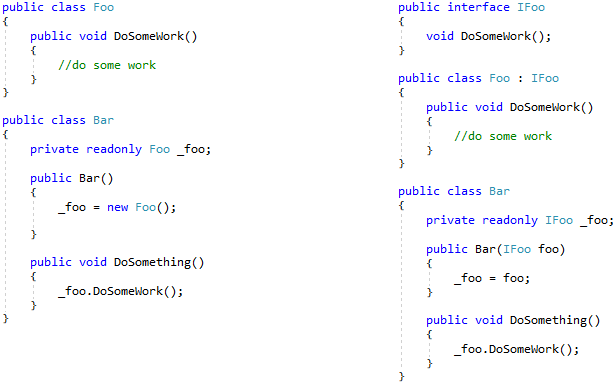
\includegraphics[height=6cm]{PresentationDIP.png}
	\end{center}
\end{figure}
\end{frame}

\subsection*{Kontenery wstrzykiwania zależności}

\begin{frame}{Kontenery wstrzykiwania zależności}
\begin{table}
     \begin{small}
	\begin{tabular}{ p{6cm} p{6cm} }
	
	\begin{minipage}{.7\textwidth}
		\begin{itemize}
			\item Rejestracja
			\item Tworzenie obiektów
		\end{itemize}
   	 \end{minipage}
	&
	\begin{minipage}{.3\textwidth}
  		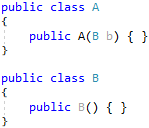
\includegraphics[height=2cm]{Example_Container.png}
\\ \\
		{\tiny \texttt{container.Register<A>();\\
			container.Register<B>();}}\\ \\
		{\tiny \texttt{container.Resolve<B>();\\
			container.Resolve<A>();}}
    	\end{minipage}
    	
	\end{tabular}
     \end{small}
\end{table}
\end{frame}

\subsection*{Obserwacje}

\begin{frame}{Obserwacje}
  \begin{itemize}
  \item W grafach zależności często powtarzają się typy
  \item Utworzenie instancji nowego obiektu zajmuje czas
  \item Nowe obiekty są często tworzone
  \end{itemize}
\end{frame}

\subsection*{Cel Pracy}

\begin{frame}{Cel Pracy}
\begin{center}
Wydajny kontener wstrzykiwania zależności
\end{center}
\end{frame}


\section{Wstrzykiwanie zależności}

\begin{frame}{}
\begin{center}
\huge{Wstrzykiwanie zależności}
\end{center}
\end{frame}

\subsection*{Wstrzykiwanie zależności}

\begin{frame}{Wstrzykiwanie zależności}
\begin{table}
     \begin{small}
	\begin{tabular}{ c p{3cm} }
	
	\begin{minipage}{.6\textwidth}
\begin{itemize}
	\item Wstrzykiwanie przez konstruktor
	\item Wstrzykiwanie przez metodę
	\item Wstrzykiwanie przez właściwość
\end{itemize}
   	 \end{minipage}
   	 &   	 
	\begin{minipage}{.4\textwidth}	
  		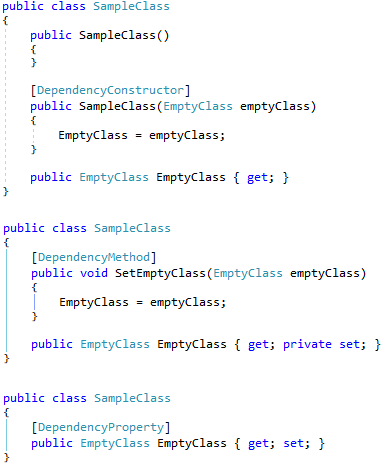
\includegraphics[height=5cm]{PresentationDependency.png}
   	 \end{minipage}

	\end{tabular}
     \end{small}
\end{table}
\end{frame}

\subsection*{Implementacje przemysłowe}

\begin{frame}{Implementacje przemysłowe}
\begin{table}
	\begin{tabular}{ p{5cm} p{5cm} }
	
	\begin{minipage}{.5\textwidth}
\begin{itemize}
	\item Unity
	\item NInject
	\item Autofac
	\item StructureMap
	\item Windsor
\end{itemize}
   	 \end{minipage}
   	 &
	\begin{minipage}{.5\textwidth}
\begin{itemize}
	\item Grace
	\item DryIoc
	\item LightInject
	\item SimpleInjector
\end{itemize}
   	 \end{minipage}

	\end{tabular}
\end{table}
\end{frame}


\section{Implementacja}

\begin{frame}{}
\begin{center}
\huge{Implementacja}
\end{center}
\end{frame}

\begin{frame}{Implementacja}
\begin{table}
     \begin{small}
	\begin{tabular}{ p{6cm} p{3cm} }
	
	\begin{minipage}{.6\textwidth}
\begin{itemize}
	\item CIL
	\item Reflection.Emit
\end{itemize}
\color{white}. \\ \\
. .
  		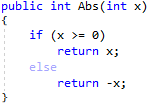
\includegraphics[height=1.5cm]{Example_Abs.png}
   	 \end{minipage}
   	 &   	 
	\begin{minipage}{.6\textwidth}
\tiny{\texttt{IL\_0000:  ldarg.1 \\
IL\_0001:  ldc.i4.0 \\
IL\_0002:  blt.s      IL\_0006 \\
IL\_0004:  ldarg.1 \\
IL\_0005:  ret \\
IL\_0006:  ldarg.1 \\
IL\_007:  neg \\
IL\_008:  ret }}
\\ \\ \\
  		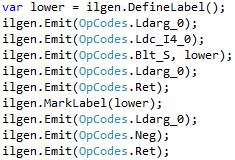
\includegraphics[height=2cm]{PresentationEmit.png}
   	 \end{minipage}

	\end{tabular}
     \end{small}
\end{table}
\end{frame}

\subsection*{Dwa rozwiązania}

\begin{frame}{Dwa rozwiązania}
\begin{itemize}
	\item Partial Emit Function
	\item Full Emit Function
\end{itemize}
\end{frame}

\subsection*{Partial Emit Function}

\begin{frame}{Partial Emit Function}
\begin{figure}[H]
	\begin{center}
  		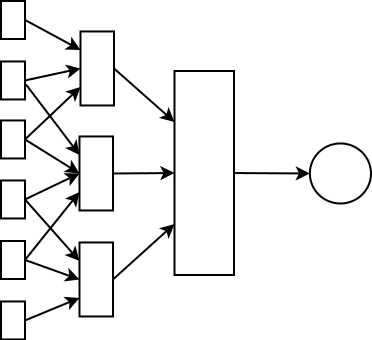
\includegraphics[height=6cm]{PresentationPartial.png}
	\end{center}
\end{figure}
\end{frame}

\subsection*{Full Emit Function}

\begin{frame}{Full Emit Function}
\begin{figure}[H]
	\begin{center}
  		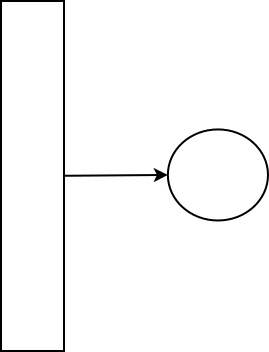
\includegraphics[height=6cm]{PresentationFull.png}
	\end{center}
\end{figure}
\end{frame}


\section{Wyniki}
\begin{frame}{}
\begin{center}
\huge{Wyniki}
\end{center}
\end{frame}

\subsection*{Przypadki testowe}

\begin{frame}{Przypadki testowe}
\begin{table}
     \begin{small}
	\begin{tabular}{ p{4cm} p{6cm} }
	
	\begin{minipage}{.5\textwidth}
\begin{figure}[H]
	\begin{center}
	  	A
  		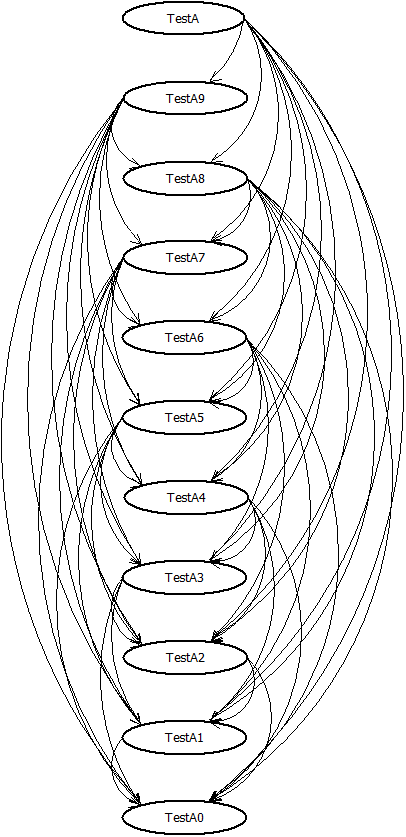
\includegraphics[height=2.5cm]{TestA.png}
	\end{center}
\end{figure}
   	 \end{minipage}
   	 &	
	\begin{minipage}{.5\textwidth}
\begin{figure}[H]
	\begin{center}
		B
  		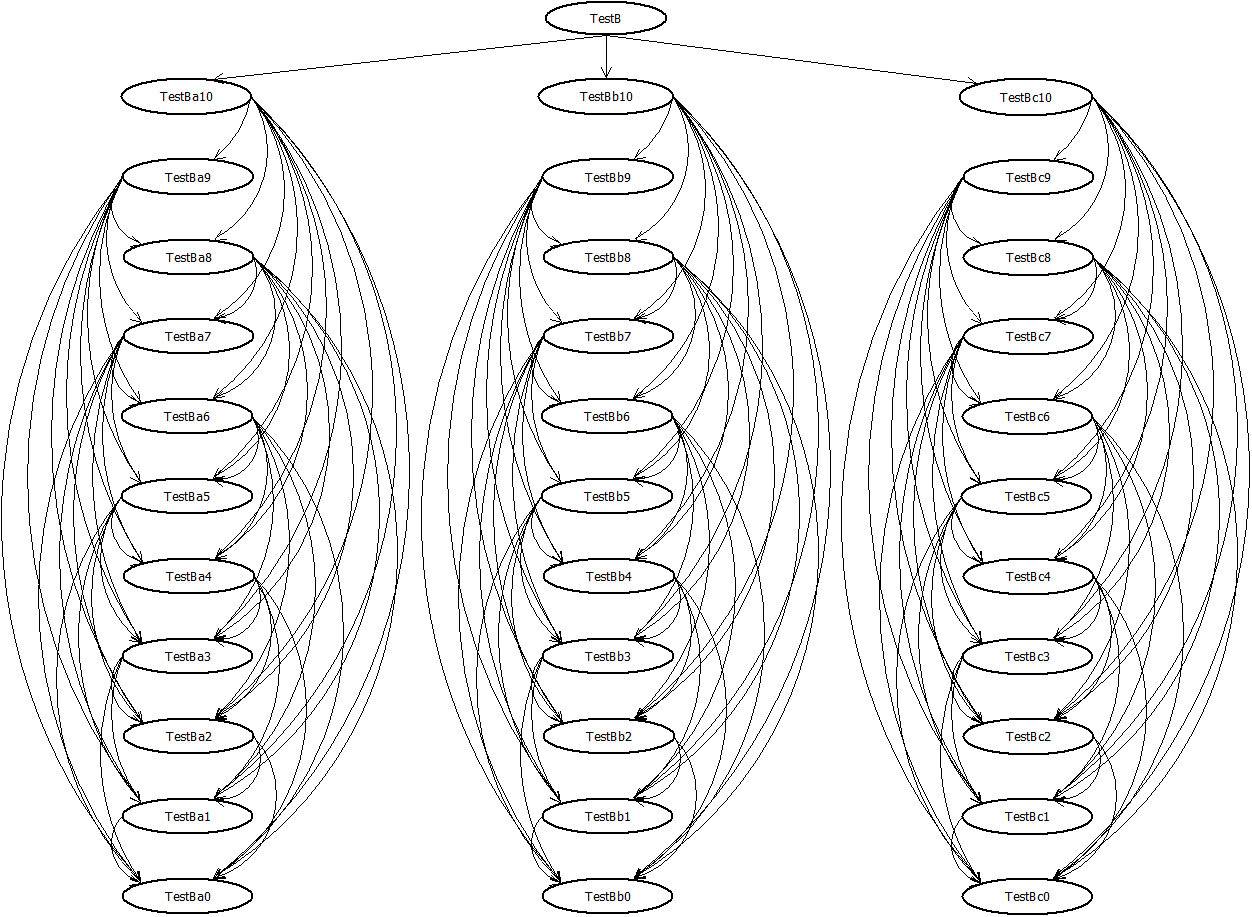
\includegraphics[height=2.5cm]{TestB.png}
	\end{center}
\end{figure}
   	 \end{minipage}
   	 \\ \\
	\begin{minipage}{.5\textwidth}
\begin{figure}[H]
	\begin{center}
		C
  		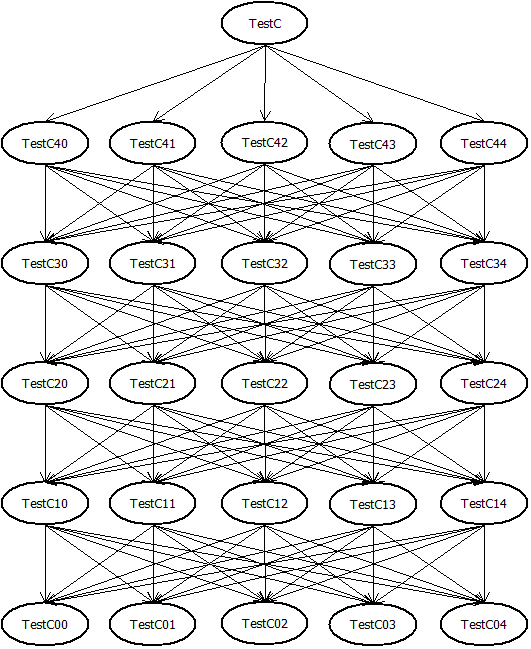
\includegraphics[height=2.5cm]{TestC.png}
	\end{center}
\end{figure}
   	 \end{minipage}
   	 &	
	\begin{minipage}{.5\textwidth}
\begin{figure}[H]
	\begin{center}
		D
  		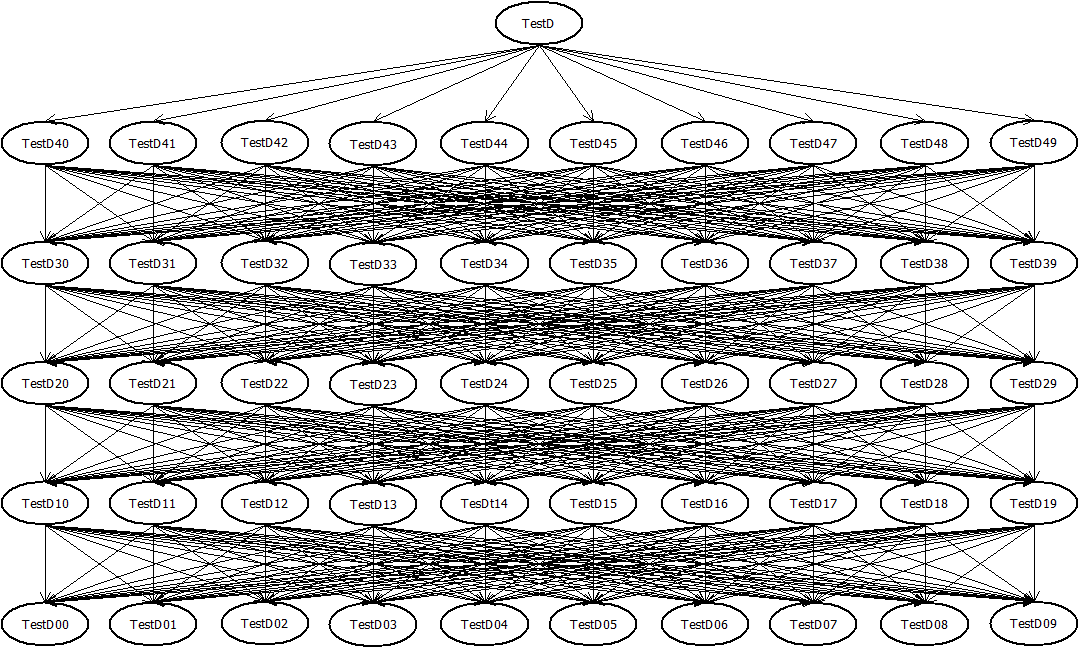
\includegraphics[height=2.5cm]{TestD.png}
	\end{center}
\end{figure}
   	 \end{minipage}

	\end{tabular}
     \end{small}
\end{table}
\end{frame}

\subsection*{Typy rejestracji}

\begin{frame}{Typy rejestracji}
\begin{itemize}
	\item Register as Singleton,
	\item Register as Transient,
	\item Register as TransientSingleton,
	\item Register as PerThread (PerScope),
	\item Register as FactoryMethod.
\end{itemize}
\end{frame}

\begin{frame}{Typy rejestracji}
\begin{itemize}
	\color{gray}
	\item Register as Singleton,
	\color{black}
	\item Register as Transient,
	\color{gray}
	\item Register as TransientSingleton,
	\item Register as PerThread (PerScope),
	\item Register as FactoryMethod.
\end{itemize}
\end{frame}

\subsection*{Przypadek testowy A}

\begin{frame}{Przypadek testowy A - graf zależności}
\begin{table}
     \begin{small}
	\begin{tabular}{ p{7cm} p{2cm} }
	
	\begin{minipage}{.7\textwidth}
\begin{figure}
	\begin{center}
  		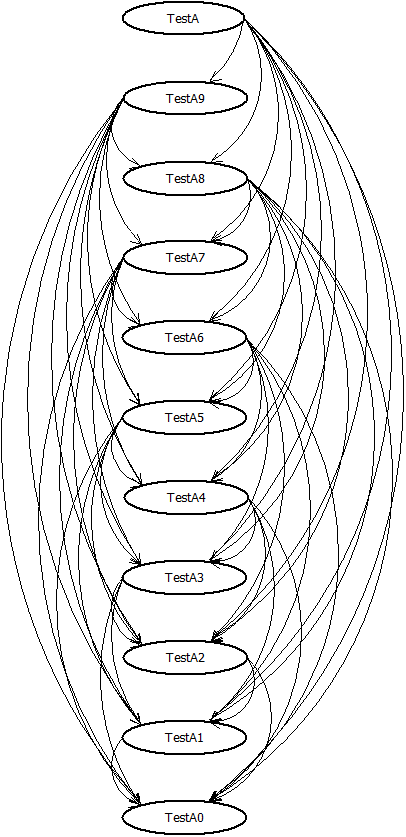
\includegraphics[height=6cm]{TestA.png}
	\end{center}
\end{figure}
   	 \end{minipage}
&
	\begin{minipage}{.3\textwidth}
\tiny{Liczba obiektów w 1 iteracji: 1 024}
   	 \end{minipage}

	\end{tabular}
     \end{small}
\end{table}
\end{frame}

\begin{frame}{Przypadek testowy A - Transient}
Liczba iteracji: 1 i 10
\begin{table}
\begin{small}
	\begin{tabular}{ l  r }
		\begin{tabular}{ | l | r | }
    		\hline
		Autofac &  0 \\ \hline
		\textbf{NiquIoCPartial}  & \textbf{1} \\ \hline
		Windsor & 1 \\ \hline
		\textbf{NiquIoCFull} & \textbf{8} \\ \hline
		Unity & 8 \\ \hline
		LightInject & 10 \\ \hline
		StructureMap & 10 \\ \hline
		Ninject & 11 \\ \hline
		SimpleInjector & 13 \\ \hline
		DryIoc & 14 \\ \hline
		Grace & 15 \\ \hline
  		\end{tabular}
	&
		\begin{tabular}{ | l | r | }
    		\hline
		\textbf{NiquIoCPartial} & \textbf{3} \\ \hline
		Autofac & 6 \\ \hline
		\textbf{NiquIoCFull} & \textbf{8} \\ \hline
		LightInject & 10 \\ \hline
		SimpleInjector & 14 \\ \hline
		StructureMap & 14 \\ \hline
		DryIoc & 15 \\ \hline
		Grace & 16 \\ \hline
		Unity & 16 \\ \hline
		Windsor & 16 \\ \hline
		Ninject & 90 \\ \hline
  		\end{tabular}
  	\end{tabular}
\end{small}
\end{table}
\end{frame}

\begin{frame}{Przypadek testowy A - Transient}
Liczba iteracji: 100 i 1000
\begin{table}
\begin{center}
\begin{small}
	\begin{tabular}{ l  r }
		\begin{tabular}{ | l | r | }
    		\hline
		\textbf{NiquIoCFull} & \textbf{9} \\ \hline
		LightInject & 11 \\ \hline
		SimpleInjector & 15 \\ \hline
		DryIoc & 16 \\ \hline
		Grace & 18 \\ \hline
		\textbf{NiquIoCPartial} & \textbf{19} \\ \hline
		StructureMap & 54 \\ \hline
		Autofac & 59 \\ \hline
		Unity & 88 \\ \hline
		Windsor & 155 \\ \hline
		Ninject & 882 \\ \hline
  		\end{tabular}
	&
		\begin{tabular}{ | l | r | }
    		\hline
		\textbf{NiquIoCFull} & \textbf{18} \\ \hline
		LightInject & 19 \\ \hline
		SimpleInjector & 29 \\ \hline
		DryIoc & 29 \\ \hline
		Grace & 37 \\ \hline
		\textbf{NiquIoCPartial} & \textbf{173} \\ \hline
		StructureMap & 417 \\ \hline
		Autofac & 587 \\ \hline
		Unity & 813 \\ \hline
		Windsor & 1529 \\ \hline
		Ninject & 8934 \\ \hline
  		\end{tabular}
  	\end{tabular}
\end{small}
\end{center}
\end{table}
\end{frame}

\subsection*{Przypadek testowy C}

\begin{frame}{Przypadek testowy C - graf zależności}
\begin{table}
     \begin{small}
	\begin{tabular}{ p{7cm} p{2cm} }
	
	\begin{minipage}{.7\textwidth}
\begin{figure}
	\begin{center}
  		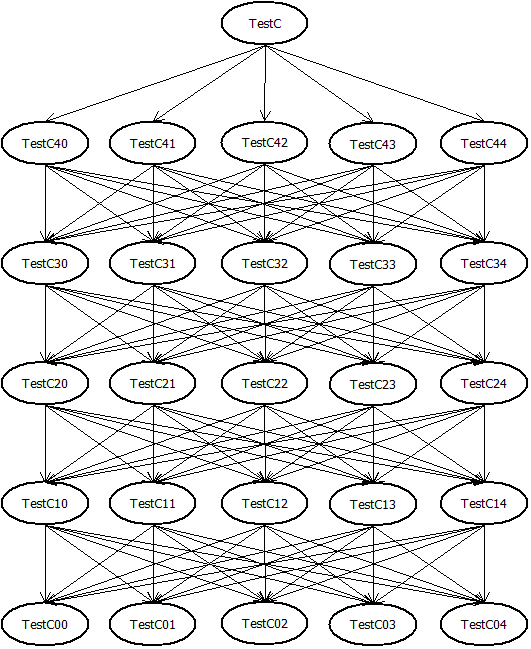
\includegraphics[height=6cm]{TestC.png}
	\end{center}
\end{figure}
   	 \end{minipage}
&
	\begin{minipage}{.3\textwidth}
\tiny{Liczba obiektów w 1 iteracji: 3 906}
   	 \end{minipage}

	\end{tabular}
     \end{small}
\end{table}
\end{frame}

\begin{frame}{Przypadek testowy C - Transient}
Liczba iteracji: 1 i 10
\begin{table}
\begin{small}
	\begin{tabular}{ l  r }
		\begin{tabular}{ | l | r | }
    		\hline
		Autofac & 2 \\ \hline
		\textbf{NiquIoCPartial} & \textbf{4} \\ \hline
		Windsor & 7 \\ \hline
		Unity & 19 \\ \hline
		StructureMap & 26 \\ \hline
		\textbf{NiquIoCFull} & \textbf{31} \\ \hline
		LightInject & 36 \\ \hline
		DryIoc & 39 \\ \hline
		Ninject & 39 \\ \hline
		SimpleInjector & 41 \\ \hline
		Grace & 61 \\ \hline
  		\end{tabular}
	&
		\begin{tabular}{ | l | r | }
    		\hline
		\textbf{NiquIoCPartial} & \textbf{10 }\\ \hline
		Autofac & 24 \\ \hline
		\textbf{NiquIoCFull} & \textbf{32} \\ \hline
		LightInject & 37 \\ \hline
		DryIoc & 40 \\ \hline
		StructureMap & 40 \\ \hline
		SimpleInjector & 41 \\ \hline
		Unity & 47 \\ \hline
		Grace & 62 \\ \hline
		Windsor & 62 \\ \hline
		Ninject & 353 \\ \hline
  		\end{tabular}
  	\end{tabular}
\end{small}
\end{table}
\end{frame}

\begin{frame}{Przypadek testowy C - Transient}
Liczba iteracji: 100 i 1000
\begin{table}
\begin{small}
	\begin{tabular}{ l  r }
		\begin{tabular}{ | l | r | }
    		\hline
		\textbf{NiquIoCFull} & \textbf{38} \\ \hline
		LightInject & 44 \\ \hline
		DryIoc & 47 \\ \hline
		SimpleInjector & 49 \\ \hline
		Grace & 73 \\ \hline
		\textbf{NiquIoCPartial} & \textbf{74} \\ \hline
		StructureMap & 181 \\ \hline
		Autofac & 231 \\ \hline
		Unity & 318 \\ \hline
		Windsor & 608 \\ \hline
		Ninject & 3511 \\ \hline
  		\end{tabular}
	&
		\begin{tabular}{ | l | r | }
    		\hline
		\textbf{NiquIoCFull} & \textbf{82} \\ \hline
		LightInject & 86 \\ \hline
		DryIoc & 99 \\ \hline
		SimpleInjector & 116 \\ \hline
		Grace & 155 \\ \hline
		\textbf{NiquIoCPartial} & \textbf{690} \\ \hline
		StructureMap & 1540 \\ \hline
		Autofac & 2288 \\ \hline
		Unity & 3015 \\ \hline
		Windsor & 6037 \\ \hline
		Ninject & 37642 \\ \hline
  		\end{tabular}
  	\end{tabular}
\end{small}
\end{table}
\end{frame}


\section{Podsumowanie}

\begin{frame}{}
\begin{center}
\huge{Podsumowanie}
\end{center}
\end{frame}

\begin{frame}{}
\begin{table}
     \begin{small}
	\begin{tabular}{ p{5cm} p{5cm} }
	
	\begin{minipage}{.5\textwidth}
	\begin{center}
  		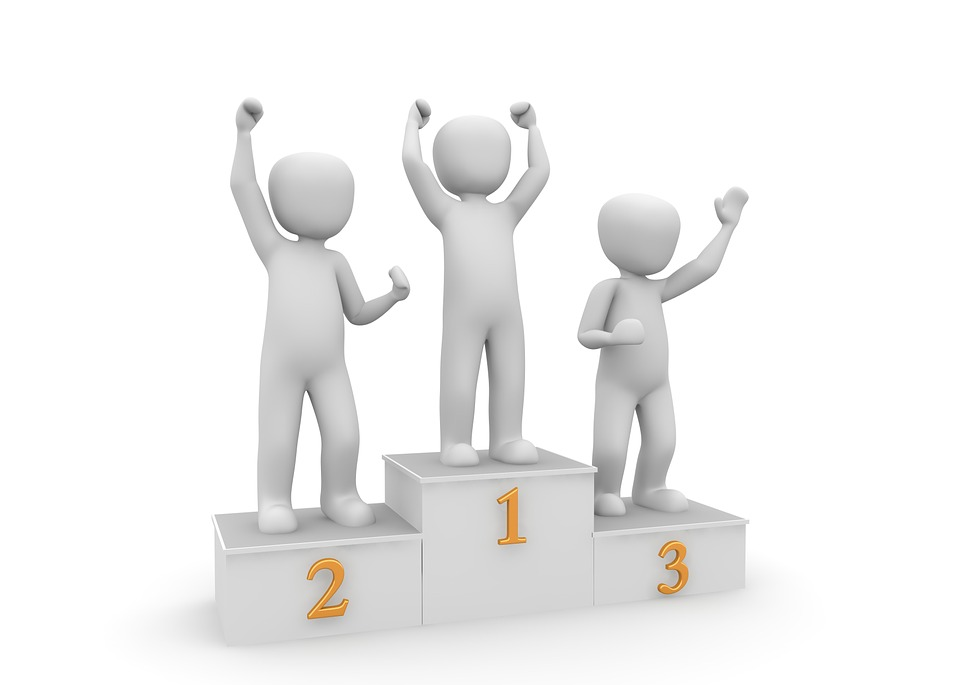
\includegraphics[height=2.5cm]{PresentationWinner.jpg}
	\end{center}
   	 \end{minipage}
   	 &	
	\begin{minipage}{.5\textwidth}	
	\begin{center}
  		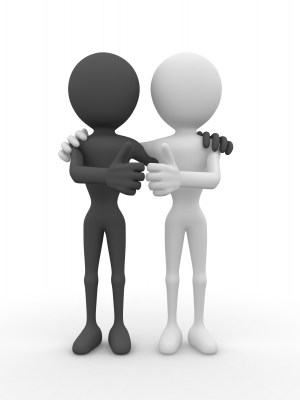
\includegraphics[height=2.5cm]{PresentationConnect.jpg}
	\end{center}
   	 \end{minipage}

	\end{tabular}
     \end{small}
\end{table}
\end{frame}

\end{document}